\documentclass[11pt, letterpaper]{article}

% Fonts and Encoding
\usepackage[utf8]{inputenc}
\usepackage[T1]{fontenc}
\usepackage{lmodern} % High-quality Latin Modern vector font

% Math and Symbols
\usepackage{amsmath, amssymb, amsthm, amsfonts, mathrsfs, mathtools}

% Layout and Geometry
\usepackage{geometry}
\geometry{letterpaper, margin=1in}
\setlength{\parindent}{0pt}
\setlength{\parskip}{0.6em}

% Formatting and Graphics
\usepackage{graphicx, xcolor, enumitem, booktabs, array, tabularx}

% TikZ for Illustrations
\usepackage{tikz}
\usetikzlibrary{arrows.meta, positioning, shapes.geometric, calc, backgrounds, matrix}

% Clickable Links and TOC
\usepackage{hyperref}
\hypersetup{
    colorlinks=true,
    linkcolor=blue,
    filecolor=magenta,      
    urlcolor=cyan,
    pdftitle={Advanced Mathematics Topic},
}

% Theorem Environments
\newtheorem{theorem}{Theorem}[section]
\newtheorem{lemma}[theorem]{Lemma}
\newtheorem{proposition}[theorem]{Proposition}
\newtheorem{corollary}[theorem]{Corollary}
\theoremstyle{definition}
\newtheorem{definition}{Definition}[section]
\newtheorem{axiom}{Axiom}[section]
\newtheorem{example}{Example}[section]
\theoremstyle{remark}
\newtheorem{remark}{Remark}[section]

% Custom Commands (Enforced standard notation)
\newcommand{\R}{\mathbb{R}}
\newcommand{\N}{\mathbb{N}}
\newcommand{\Z}{\mathbb{Z}}
\newcommand{\Q}{\mathbb{Q}}
\newcommand{\E}{\mathbb{E}}
\newcommand{\Prob}{\mathbb{P}}
\newcommand{\F}{\mathcal{F}}

\title{Mastering Convolution and the Dirac Delta Function\\ \Large Comprehensive Problem Sets and Solutions}
\author{Tashfeen Omran}
\date{\today}

\begin{document}

\maketitle
\tableofcontents
\newpage

\section{Concept Checklist \& Question Mapping}

To ensure comprehensive coverage of the topics presented in the source material, the following concepts have been identified and mapped to specific problems in this document. A total of 32 problems have been curated to test these concepts rigorously.

\renewcommand{\arraystretch}{1.5}
\begin{tabularx}{\textwidth}{>{\raggedright\arraybackslash}X >{\centering\arraybackslash}c}
\toprule
\textbf{Concept / Problem Type} & \textbf{Associated Questions} \\
\midrule
\textbf{Concept 1:} Direct Computation of Convolution Integrals & 1, 2, 3, 4 \\
\textbf{Concept 2:} Inverse Laplace Transforms via Convolution & 5, 6, 7, 8, 9, 10 \\
\textbf{Concept 3:} Solving Integro-Differential Equations & 11, 12, 13, 14, 15, 16 \\
\textbf{Concept 4:} Initial Value Problems with General Forcing Functions & 17, 18, 19, 20, 21 \\
\textbf{Concept 5:} Transfer Functions and Impulse Responses & 22, 23, 24, 25 \\
\textbf{Concept 6:} Convolution with Dirac Delta and Heaviside Functions & 26, 27, 28 \\
\textbf{Concept 7:} Discrete Convolution & 29, 30 \\
\textbf{Concept 8:} Advanced Diagnostic Testing (``Find the Flaw'') & 31, 32 \\
\bottomrule
\end{tabularx}

\vspace{1em}
\begin{center}
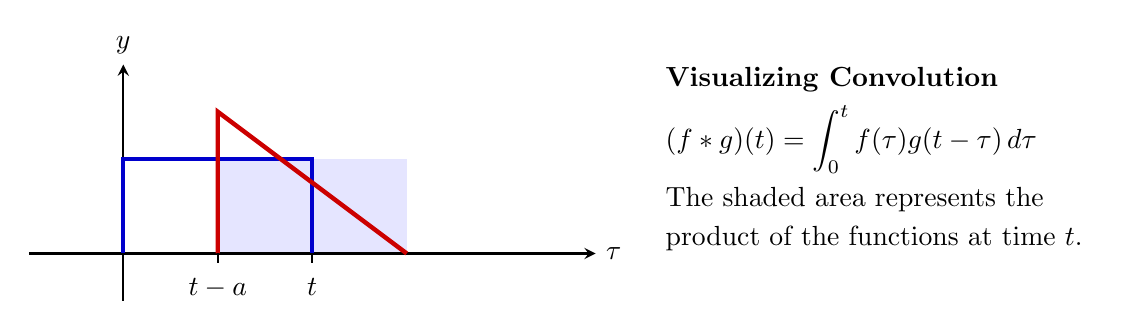
\begin{tikzpicture}[scale=1.2]
    % 1) Backgrounds
    \fill[blue!10] (1,0) rectangle (3,1);
    
    % 2) Grids/Axes
    \draw[thick, ->, >=stealth] (-1,0) -- (5,0) node[right] {$\tau$};
    \draw[thick, ->, >=stealth] (0,-0.5) -- (0,2) node[above] {$y$};
    
    % 3) Primary Plots
    \draw[ultra thick, blue!80!black] (0,0) -- (0,1) -- (2,1) -- (2,0);
    \draw[ultra thick, red!80!black] (1,0) -- (1,1.5) -- (3,0);
    
    % 4) Nodes/Labels
    \node[align=left, inner sep=8pt, anchor=west] at (5.5, 1) {
        \textbf{Visualizing Convolution}\\[4pt]
        $\displaystyle (f * g)(t) = \int_0^t f(\tau)g(t-\tau) \, d\tau$\\[4pt]
        The shaded area represents the\\[2pt]
        product of the functions at time $t$.
    };
    \draw[thick] (2,0) -- (2,-0.1) node[below=2pt] {$t$};
    \draw[thick] (1,0) -- (1,-0.1) node[below=2pt] {$t-a$};
\end{tikzpicture}
\end{center}

\newpage

\section{Problem Sets}

\subsection{Concept 1: Direct Computation of Convolution Integrals}
Compute the following convolutions directly using the definition $(f * g)(t) = \int_0^t f(t-v)g(v) \, dv$.
\begin{enumerate}[label=\textbf{\arabic*.}]
    \item $f(t) = t$, $g(t) = t$
    \item $f(t) = e^{2t}$, $g(t) = e^{-t}$
    \item $f(t) = \sin(t)$, $g(t) = \cos(t)$
    \item $f(t) = 1$, $g(t) = t^3$
\end{enumerate}

\subsection{Concept 2: Inverse Laplace Transforms via Convolution}
Use the Convolution Theorem, $\mathcal{L}^{-1}\{F(s)G(s)\} = (f * g)(t)$, to find the inverse Laplace transform of the following functions.
\begin{enumerate}[label=\textbf{\arabic*.}, resume]
    \item $\displaystyle Y(s) = \frac{1}{s^2(s-2)}$
    \item $\displaystyle Y(s) = \frac{s}{(s^2+4)^2}$
    \item $\displaystyle Y(s) = \frac{1}{(s-1)(s-3)}$
    \item $\displaystyle Y(s) = \frac{1}{s(s^2+9)}$
    \item $\displaystyle Y(s) = \frac{1}{(s^2+1)^2}$
    \item $\displaystyle Y(s) = \frac{s}{(s^2+1)(s^2+4)}$
\end{enumerate}

\subsection{Concept 3: Solving Integro-Differential Equations}
Solve the following integral and integro-differential equations using the Laplace transform.
\begin{enumerate}[label=\textbf{\arabic*.}, resume]
    \item $\displaystyle y(t) + \int_0^t y(v) \, dv = t$
    \item $\displaystyle y(t) - 3 \int_0^t e^{2(t-v)}y(v) \, dv = e^t$
    \item $\displaystyle y'(t) + \int_0^t y(v)\cos(t-v) \, dv = 1, \quad y(0) = 0$
    \item $\displaystyle y(t) = t^2 + \int_0^t y(v)\sin(t-v) \, dv$
    \item $\displaystyle y'(t) - \int_0^t (t-v)y(v) \, dv = t, \quad y(0) = 1$
    \item $\displaystyle y(t) + 4 \int_0^t (t-v)^2 y(v) \, dv = t^3$
\end{enumerate}

\subsection{Concept 4: Initial Value Problems with General Forcing Functions}
Solve the following initial value problems in terms of a convolution integral with the arbitrary forcing function $g(t)$.
\begin{enumerate}[label=\textbf{\arabic*.}, resume]
    \item $y'' + 16y = g(t), \quad y(0) = 1, \quad y'(0) = 0$
    \item $y'' - 4y' + 4y = g(t), \quad y(0) = 0, \quad y'(0) = 2$
    \item $y'' + 2y' + 2y = g(t), \quad y(0) = 0, \quad y'(0) = 0$
    \item $y'' - y = g(t), \quad y(0) = -1, \quad y'(0) = 1$
    \item $y'' + 6y' + 9y = g(t), \quad y(0) = 2, \quad y'(0) = -6$
\end{enumerate}

\subsection{Concept 5: Transfer Functions and Impulse Responses}
For each of the following systems, find the transfer function $H(s)$ and the impulse response $h(t)$.
\begin{enumerate}[label=\textbf{\arabic*.}, resume]
    \item $y'' + 7y' + 10y = g(t)$
    \item $y'' + 4y' + 13y = g(t)$
    \item $2y'' + 8y' + 8y = g(t)$
    \item $y''' - y'' = g(t)$
\end{enumerate}

\subsection{Concept 6: Convolution with Dirac Delta and Heaviside Functions}
Evaluate the following expressions involving the Dirac delta function $\delta(t)$.
\begin{enumerate}[label=\textbf{\arabic*.}, resume]
    \item Evaluate $y(t) = e^{3t} * \delta(t-2)$.
    \item Evaluate $y(t) = \cos(t) * \delta(t-\pi/2)$.
    \item Solve the initial value problem: $y'' + 4y = \delta(t-\pi), \quad y(0) = 0, \quad y'(0) = 0$.
\end{enumerate}

\subsection{Concept 7: Discrete Convolution}
Compute the discrete convolution $(f * g)[n] = \sum_{m=-\infty}^{\infty} f[m]g[n-m]$ for the following sequences (assume sequences start at $n=0$).
\begin{enumerate}[label=\textbf{\arabic*.}, resume]
    \item $f = [2, -1, 3]$ and $g = [1, 2]$
    \item $f = [1, 1, 1]$ and $g = [1, -1]$
\end{enumerate}

\subsection{Concept 8: Advanced Diagnostic Testing (``Find the Flaw'')}
Identify the conceptual or mathematical flaw in the following proposed solutions and provide the correct solution.
\begin{enumerate}[label=\textbf{\arabic*.}, resume]
    \item \textbf{Problem:} Find $\mathcal{L}^{-1}\left\{\frac{1}{s(s-3)}\right\}$.\\
    \textbf{Flawed Solution:} $\mathcal{L}^{-1}\left\{\frac{1}{s}\right\} = 1$ and $\mathcal{L}^{-1}\left\{\frac{1}{s-3}\right\} = e^{3t}$. Therefore, the inverse transform is $1 \cdot e^{3t} = e^{3t}$.
    \item \textbf{Problem:} Evaluate $t * t^2$.\\
    \textbf{Flawed Solution:} $t * t^2 = \int_0^\infty (t-v)v^2 \, dv = \left[ \frac{tv^3}{3} - \frac{v^4}{4} \right]_0^\infty = \infty$.
\end{enumerate}

\newpage

\section{Detailed Solutions}

\subsection{Concept 1: Direct Computation of Convolution Integrals}

\textbf{Problem 1:} Compute $f(t) = t$, $g(t) = t$.
\vspace{0.5em}\\
\textbf{Solution:}
By the definition of convolution:
\[ (t * t) = \int_0^t (t-v)v \, dv = \int_0^t (tv - v^2) \, dv \]
Integrating with respect to $v$:
\[ = \left[ t\frac{v^2}{2} - \frac{v^3}{3} \right]_0^t = \frac{t^3}{2} - \frac{t^3}{3} = \frac{t^3}{6} \]

\textbf{Problem 2:} Compute $f(t) = e^{2t}$, $g(t) = e^{-t}$.
\vspace{0.5em}\\
\textbf{Solution:}
\[ (e^{2t} * e^{-t}) = \int_0^t e^{2(t-v)}e^{-v} \, dv = \int_0^t e^{2t}e^{-2v}e^{-v} \, dv = e^{2t} \int_0^t e^{-3v} \, dv \]
\[ = e^{2t} \left[ \frac{e^{-3v}}{-3} \right]_0^t = e^{2t} \left( \frac{e^{-3t} - 1}{-3} \right) = \frac{1}{3}(e^{2t} - e^{-t}) \]

\textbf{Problem 3:} Compute $f(t) = \sin(t)$, $g(t) = \cos(t)$.
\vspace{0.5em}\\
\textbf{Solution:}
\[ (\sin(t) * \cos(t)) = \int_0^t \sin(t-v)\cos(v) \, dv \]
Using the product-to-sum identity $\sin(A)\cos(B) = \frac{1}{2}[\sin(A+B) + \sin(A-B)]$:
\[ = \frac{1}{2} \int_0^t [\sin(t) + \sin(t-2v)] \, dv \]
\[ = \frac{1}{2} \left[ v\sin(t) + \frac{\cos(t-2v)}{2} \right]_0^t \]
\[ = \frac{1}{2} \left( t\sin(t) + \frac{\cos(-t)}{2} - \frac{\cos(t)}{2} \right) = \frac{1}{2}t\sin(t) \]

\textbf{Problem 4:} Compute $f(t) = 1$, $g(t) = t^3$.
\vspace{0.5em}\\
\textbf{Solution:}
\[ (1 * t^3) = \int_0^t 1 \cdot v^3 \, dv = \left[ \frac{v^4}{4} \right]_0^t = \frac{t^4}{4} \]

\subsection{Concept 2: Inverse Laplace Transforms via Convolution}

\textbf{Problem 5:} Find $\mathcal{L}^{-1}\left\{\frac{1}{s^2(s-2)}\right\}$.
\vspace{0.5em}\\
\textbf{Solution:}
Let $F(s) = \frac{1}{s^2}$ and $G(s) = \frac{1}{s-2}$. Then $f(t) = t$ and $g(t) = e^{2t}$.
\[ \mathcal{L}^{-1}\{F(s)G(s)\} = t * e^{2t} = \int_0^t (t-v)e^{2v} \, dv \]
Using integration by parts, let $u = t-v \implies du = -dv$, and $dw = e^{2v}dv \implies w = \frac{1}{2}e^{2v}$:
\[ = \left[ (t-v)\frac{1}{2}e^{2v} \right]_0^t - \int_0^t -\frac{1}{2}e^{2v} \, dv \]
\[ = \left( 0 - \frac{t}{2} \right) + \left[ \frac{1}{4}e^{2v} \right]_0^t = -\frac{t}{2} + \frac{1}{4}e^{2t} - \frac{1}{4} \]

\textbf{Problem 6:} Find $\mathcal{L}^{-1}\left\{\frac{s}{(s^2+4)^2}\right\}$.
\vspace{0.5em}\\
\textbf{Solution:}
Let $F(s) = \frac{s}{s^2+4}$ and $G(s) = \frac{1}{s^2+4}$. Then $f(t) = \cos(2t)$ and $g(t) = \frac{1}{2}\sin(2t)$.
\[ \mathcal{L}^{-1}\{F(s)G(s)\} = \cos(2t) * \frac{1}{2}\sin(2t) = \frac{1}{2} \int_0^t \cos(2(t-v))\sin(2v) \, dv \]
Using $\cos(A)\sin(B) = \frac{1}{2}[\sin(A+B) - \sin(A-B)]$:
\[ = \frac{1}{4} \int_0^t [\sin(2t) - \sin(2t-4v)] \, dv \]
\[ = \frac{1}{4} \left[ v\sin(2t) - \frac{\cos(2t-4v)}{4} \right]_0^t \]
\[ = \frac{1}{4} \left( t\sin(2t) - \frac{\cos(-2t)}{4} + \frac{\cos(2t)}{4} \right) = \frac{1}{4}t\sin(2t) \]

\textbf{Problem 7:} Find $\mathcal{L}^{-1}\left\{\frac{1}{(s-1)(s-3)}\right\}$.
\vspace{0.5em}\\
\textbf{Solution:}
Let $F(s) = \frac{1}{s-1}$ and $G(s) = \frac{1}{s-3}$. Then $f(t) = e^t$ and $g(t) = e^{3t}$.
\[ e^t * e^{3t} = \int_0^t e^{t-v}e^{3v} \, dv = e^t \int_0^t e^{2v} \, dv = e^t \left[ \frac{1}{2}e^{2v} \right]_0^t = \frac{1}{2}e^t(e^{2t} - 1) = \frac{1}{2}(e^{3t} - e^t) \]

\textbf{Problem 8:} Find $\mathcal{L}^{-1}\left\{\frac{1}{s(s^2+9)}\right\}$.
\vspace{0.5em}\\
\textbf{Solution:}
Let $F(s) = \frac{1}{s}$ and $G(s) = \frac{1}{s^2+9}$. Then $f(t) = 1$ and $g(t) = \frac{1}{3}\sin(3t)$.
\[ 1 * \frac{1}{3}\sin(3t) = \frac{1}{3} \int_0^t \sin(3v) \, dv = \frac{1}{3} \left[ -\frac{1}{3}\cos(3v) \right]_0^t = \frac{1}{9}(1 - \cos(3t)) \]

\textbf{Problem 9:} Find $\mathcal{L}^{-1}\left\{\frac{1}{(s^2+1)^2}\right\}$.
\vspace{0.5em}\\
\textbf{Solution:}
Let $F(s) = G(s) = \frac{1}{s^2+1}$. Then $f(t) = g(t) = \sin(t)$.
\[ \sin(t) * \sin(t) = \int_0^t \sin(t-v)\sin(v) \, dv \]
Using $\sin(A)\sin(B) = \frac{1}{2}[\cos(A-B) - \cos(A+B)]$:
\[ = \frac{1}{2} \int_0^t [\cos(t-2v) - \cos(t)] \, dv = \frac{1}{2} \left[ -\frac{\sin(t-2v)}{2} - v\cos(t) \right]_0^t \]
\[ = \frac{1}{2} \left( \frac{\sin(t)}{2} - t\cos(t) + \frac{\sin(t)}{2} \right) = \frac{1}{2}(\sin(t) - t\cos(t)) \]

\textbf{Problem 10:} Find $\mathcal{L}^{-1}\left\{\frac{s}{(s^2+1)(s^2+4)}\right\}$.
\vspace{0.5em}\\
\textbf{Solution:}
Let $F(s) = \frac{s}{s^2+1}$ and $G(s) = \frac{1}{s^2+4}$. Then $f(t) = \cos(t)$ and $g(t) = \frac{1}{2}\sin(2t)$.
\[ \cos(t) * \frac{1}{2}\sin(2t) = \frac{1}{2} \int_0^t \cos(t-v)\sin(2v) \, dv \]
Using $\cos(A)\sin(B) = \frac{1}{2}[\sin(A+B) - \sin(A-B)]$:
\[ = \frac{1}{4} \int_0^t [\sin(t+v) + \sin(3v-t)] \, dv = \frac{1}{4} \left[ -\cos(t+v) - \frac{1}{3}\cos(3v-t) \right]_0^t \]
\[ = \frac{1}{4} \left( -\cos(2t) - \frac{1}{3}\cos(2t) + \cos(t) + \frac{1}{3}\cos(-t) \right) = \frac{1}{4} \left( -\frac{4}{3}\cos(2t) + \frac{4}{3}\cos(t) \right) = \frac{1}{3}(\cos(t) - \cos(2t)) \]

\subsection{Concept 3: Solving Integro-Differential Equations}

\textbf{Problem 11:} Solve $y(t) + \int_0^t y(v) \, dv = t$.
\vspace{0.5em}\\
\textbf{Solution:}
Take the Laplace transform of both sides:
\[ Y(s) + Y(s)\frac{1}{s} = \frac{1}{s^2} \implies Y(s)\left(\frac{s+1}{s}\right) = \frac{1}{s^2} \]
\[ Y(s) = \frac{1}{s(s+1)} = \frac{1}{s} - \frac{1}{s+1} \]
Taking the inverse Laplace transform:
\[ y(t) = 1 - e^{-t} \]

\textbf{Problem 12:} Solve $y(t) - 3 \int_0^t e^{2(t-v)}y(v) \, dv = e^t$.
\vspace{0.5em}\\
\textbf{Solution:}
Take the Laplace transform:
\[ Y(s) - 3Y(s)\left(\frac{1}{s-2}\right) = \frac{1}{s-1} \implies Y(s)\left(\frac{s-5}{s-2}\right) = \frac{1}{s-1} \]
\[ Y(s) = \frac{s-2}{(s-1)(s-5)} \]
Using partial fraction decomposition:
\[ \frac{s-2}{(s-1)(s-5)} = \frac{A}{s-1} + \frac{B}{s-5} \]
$A = \frac{1-2}{1-5} = \frac{1}{4}$ and $B = \frac{5-2}{5-1} = \frac{3}{4}$.
\[ Y(s) = \frac{1/4}{s-1} + \frac{3/4}{s-5} \implies y(t) = \frac{1}{4}e^t + \frac{3}{4}e^{5t} \]

\textbf{Problem 13:} Solve $y'(t) + \int_0^t y(v)\cos(t-v) \, dv = 1, \quad y(0) = 0$.
\vspace{0.5em}\\
\textbf{Solution:}
Take the Laplace transform:
\[ sY(s) - 0 + Y(s)\left(\frac{s}{s^2+1}\right) = \frac{1}{s} \implies Y(s)\left(s + \frac{s}{s^2+1}\right) = \frac{1}{s} \]
\[ Y(s)\left(\frac{s^3+2s}{s^2+1}\right) = \frac{1}{s} \implies Y(s) = \frac{s^2+1}{s^2(s^2+2)} \]
Decompose into partial fractions:
\[ \frac{s^2+1}{s^2(s^2+2)} = \frac{A}{s} + \frac{B}{s^2} + \frac{Cs+D}{s^2+2} \]
By inspection, $A=0, C=0$. Let $u = s^2$: $\frac{u+1}{u(u+2)} = \frac{1/2}{u} + \frac{1/2}{u+2}$.
\[ Y(s) = \frac{1/2}{s^2} + \frac{1/2}{s^2+2} = \frac{1}{2}\frac{1}{s^2} + \frac{1}{2\sqrt{2}}\frac{\sqrt{2}}{s^2+2} \]
\[ y(t) = \frac{1}{2}t + \frac{1}{2\sqrt{2}}\sin(\sqrt{2}t) \]

\textbf{Problem 14:} Solve $y(t) = t^2 + \int_0^t y(v)\sin(t-v) \, dv$.
\vspace{0.5em}\\
\textbf{Solution:}
Take the Laplace transform:
\[ Y(s) = \frac{2}{s^3} + Y(s)\left(\frac{1}{s^2+1}\right) \implies Y(s)\left(1 - \frac{1}{s^2+1}\right) = \frac{2}{s^3} \]
\[ Y(s)\left(\frac{s^2}{s^2+1}\right) = \frac{2}{s^3} \implies Y(s) = \frac{2(s^2+1)}{s^5} = \frac{2}{s^3} + \frac{2}{s^5} \]
Taking the inverse Laplace transform:
\[ y(t) = t^2 + \frac{2}{24}t^4 = t^2 + \frac{1}{12}t^4 \]

\textbf{Problem 15:} Solve $y'(t) - \int_0^t (t-v)y(v) \, dv = t, \quad y(0) = 1$.
\vspace{0.5em}\\
\textbf{Solution:}
Take the Laplace transform:
\[ sY(s) - 1 - Y(s)\left(\frac{1}{s^2}\right) = \frac{1}{s^2} \implies Y(s)\left(\frac{s^3-1}{s^2}\right) = \frac{s^2+1}{s^2} \]
\[ Y(s) = \frac{s^2+1}{s^3-1} = \frac{s^2+1}{(s-1)(s^2+s+1)} \]
Partial fractions:
\[ \frac{s^2+1}{(s-1)(s^2+s+1)} = \frac{A}{s-1} + \frac{Bs+C}{s^2+s+1} \]
$A = \frac{1^2+1}{1^2+1+1} = \frac{2}{3}$.
$s^2+1 = \frac{2}{3}(s^2+s+1) + (Bs+C)(s-1)$.
At $s=0$: $1 = \frac{2}{3} - C \implies C = -\frac{1}{3}$.
Comparing $s^2$ coefficients: $1 = \frac{2}{3} + B \implies B = \frac{1}{3}$.
\[ Y(s) = \frac{2/3}{s-1} + \frac{\frac{1}{3}s - \frac{1}{3}}{s^2+s+1} = \frac{2/3}{s-1} + \frac{1}{3} \frac{s - 1}{(s+1/2)^2 + 3/4} \]
Rewrite the second term to match the shifted transform:
\[ \frac{1}{3} \frac{(s+1/2) - 3/2}{(s+1/2)^2 + 3/4} = \frac{1}{3} \frac{s+1/2}{(s+1/2)^2 + 3/4} - \frac{1}{2} \frac{1}{(s+1/2)^2 + 3/4} \]
\[ y(t) = \frac{2}{3}e^t + \frac{1}{3}e^{-t/2}\cos\left(\frac{\sqrt{3}}{2}t\right) - \frac{1}{\sqrt{3}}e^{-t/2}\sin\left(\frac{\sqrt{3}}{2}t\right) \]

\textbf{Problem 16:} Solve $y(t) + 4 \int_0^t (t-v)^2 y(v) \, dv = t^3$.
\vspace{0.5em}\\
\textbf{Solution:}
Take the Laplace transform:
\[ Y(s) + 4Y(s)\left(\frac{2}{s^3}\right) = \frac{6}{s^4} \implies Y(s)\left(\frac{s^3+8}{s^3}\right) = \frac{6}{s^4} \]
\[ Y(s) = \frac{6}{s(s^3+8)} = \frac{6}{s(s+2)(s^2-2s+4)} \]
By partial fractions:
\[ \frac{6}{s(s^3+8)} = \frac{A}{s} + \frac{B}{s+2} + \frac{Cs+D}{s^2-2s+4} \]
$A = \frac{6}{8} = \frac{3}{4}$. $B = \frac{6}{-2((-2)^2-2(-2)+4)} = \frac{6}{-2(12)} = -\frac{1}{4}$.
$6 = \frac{3}{4}(s^3+8) - \frac{1}{4}s(s^2-2s+4) + (Cs+D)s(s+2)$.
Comparing $s^3$ coefficients: $0 = \frac{3}{4} - \frac{1}{4} + C \implies C = -\frac{1}{2}$.
Comparing $s^2$ coefficients: $0 = 0 - \frac{1}{4}(-2) + 2C + D \implies 0 = \frac{1}{2} - 1 + D \implies D = \frac{1}{2}$.
\[ Y(s) = \frac{3/4}{s} - \frac{1/4}{s+2} - \frac{1}{2} \frac{s-1}{(s-1)^2+3} \]
\[ y(t) = \frac{3}{4} - \frac{1}{4}e^{-2t} - \frac{1}{2}e^t\cos(\sqrt{3}t) \]

\subsection{Concept 4: Initial Value Problems with General Forcing Functions}

\textbf{Problem 17:} Solve $y'' + 16y = g(t), \quad y(0) = 1, \quad y'(0) = 0$.
\vspace{0.5em}\\
\textbf{Solution:}
\[ s^2Y(s) - s + 16Y(s) = G(s) \implies (s^2+16)Y(s) = s + G(s) \]
\[ Y(s) = \frac{s}{s^2+16} + \frac{G(s)}{s^2+16} \]
Taking the inverse Laplace transform:
\[ y(t) = \cos(4t) + \frac{1}{4} \int_0^t \sin(4(t-v))g(v) \, dv \]

\textbf{Problem 18:} Solve $y'' - 4y' + 4y = g(t), \quad y(0) = 0, \quad y'(0) = 2$.
\vspace{0.5em}\\
\textbf{Solution:}
\[ [s^2Y(s) - 2] - 4[sY(s)] + 4Y(s) = G(s) \implies (s^2-4s+4)Y(s) = 2 + G(s) \]
\[ Y(s) = \frac{2}{(s-2)^2} + \frac{G(s)}{(s-2)^2} \]
Taking the inverse Laplace transform:
\[ y(t) = 2te^{2t} + \int_0^t (t-v)e^{2(t-v)}g(v) \, dv \]

\textbf{Problem 19:} Solve $y'' + 2y' + 2y = g(t), \quad y(0) = 0, \quad y'(0) = 0$.
\vspace{0.5em}\\
\textbf{Solution:}
\[ (s^2+2s+2)Y(s) = G(s) \implies Y(s) = \frac{G(s)}{(s+1)^2+1} \]
Taking the inverse Laplace transform:
\[ y(t) = \int_0^t e^{-(t-v)}\sin(t-v)g(v) \, dv \]

\textbf{Problem 20:} Solve $y'' - y = g(t), \quad y(0) = -1, \quad y'(0) = 1$.
\vspace{0.5em}\\
\textbf{Solution:}
\[ [s^2Y(s) + s - 1] - Y(s) = G(s) \implies (s^2-1)Y(s) = -s + 1 + G(s) \]
\[ Y(s) = \frac{-(s-1)}{(s-1)(s+1)} + \frac{G(s)}{s^2-1} = \frac{-1}{s+1} + \frac{G(s)}{s^2-1} \]
Taking the inverse Laplace transform:
\[ y(t) = -e^{-t} + \int_0^t \sinh(t-v)g(v) \, dv \]

\textbf{Problem 21:} Solve $y'' + 6y' + 9y = g(t), \quad y(0) = 2, \quad y'(0) = -6$.
\vspace{0.5em}\\
\textbf{Solution:}
\[ [s^2Y(s) - 2s + 6] + 6[sY(s) - 2] + 9Y(s) = G(s) \]
\[ (s^2+6s+9)Y(s) - 2s - 6 = G(s) \implies (s+3)^2Y(s) = 2(s+3) + G(s) \]
\[ Y(s) = \frac{2}{s+3} + \frac{G(s)}{(s+3)^2} \]
Taking the inverse Laplace transform:
\[ y(t) = 2e^{-3t} + \int_0^t (t-v)e^{-3(t-v)}g(v) \, dv \]

\subsection{Concept 5: Transfer Functions and Impulse Responses}

\textbf{Problem 22:} Find $H(s)$ and $h(t)$ for $y'' + 7y' + 10y = g(t)$.
\vspace{0.5em}\\
\textbf{Solution:}
Assuming zero initial conditions, $Y(s)(s^2+7s+10) = G(s)$.
\[ H(s) = \frac{Y(s)}{G(s)} = \frac{1}{s^2+7s+10} = \frac{1}{(s+2)(s+5)} \]
By partial fractions: $H(s) = \frac{1/3}{s+2} - \frac{1/3}{s+5}$.
\[ h(t) = \frac{1}{3}(e^{-2t} - e^{-5t}) \]

\textbf{Problem 23:} Find $H(s)$ and $h(t)$ for $y'' + 4y' + 13y = g(t)$.
\vspace{0.5em}\\
\textbf{Solution:}
\[ H(s) = \frac{1}{s^2+4s+13} = \frac{1}{(s+2)^2+9} \]
\[ h(t) = \frac{1}{3}e^{-2t}\sin(3t) \]

\textbf{Problem 24:} Find $H(s)$ and $h(t)$ for $2y'' + 8y' + 8y = g(t)$.
\vspace{0.5em}\\
\textbf{Solution:}
\[ H(s) = \frac{1}{2s^2+8s+8} = \frac{1}{2(s^2+4s+4)} = \frac{1}{2(s+2)^2} \]
\[ h(t) = \frac{1}{2}te^{-2t} \]

\textbf{Problem 25:} Find $H(s)$ and $h(t)$ for $y''' - y'' = g(t)$.
\vspace{0.5em}\\
\textbf{Solution:}
\[ H(s) = \frac{1}{s^3-s^2} = \frac{1}{s^2(s-1)} \]
By partial fractions: $H(s) = \frac{1}{s-1} - \frac{1}{s} - \frac{1}{s^2}$.
\[ h(t) = e^t - 1 - t \]

\subsection{Concept 6: Convolution with Dirac Delta and Heaviside Functions}

\textbf{Problem 26:} Evaluate $y(t) = e^{3t} * \delta(t-2)$.
\vspace{0.5em}\\
\textbf{Solution:}
By the sifting property of the Dirac delta function, $f(t) * \delta(t-a) = f(t-a)u(t-a)$.
\[ y(t) = e^{3(t-2)}u(t-2) \]

\textbf{Problem 27:} Evaluate $y(t) = \cos(t) * \delta(t-\pi/2)$.
\vspace{0.5em}\\
\textbf{Solution:}
\[ y(t) = \cos(t-\pi/2)u(t-\pi/2) = \sin(t)u(t-\pi/2) \]

\textbf{Problem 28:} Solve $y'' + 4y = \delta(t-\pi), \quad y(0) = 0, \quad y'(0) = 0$.
\vspace{0.5em}\\
\textbf{Solution:}
Take the Laplace transform:
\[ (s^2+4)Y(s) = e^{-\pi s} \implies Y(s) = e^{-\pi s} \frac{1}{s^2+4} \]
The inverse transform of $\frac{1}{s^2+4}$ is $\frac{1}{2}\sin(2t)$. Using the second shifting theorem:
\[ y(t) = \frac{1}{2}\sin(2(t-\pi))u(t-\pi) = \frac{1}{2}\sin(2t-2\pi)u(t-\pi) = \frac{1}{2}\sin(2t)u(t-\pi) \]

\subsection{Concept 7: Discrete Convolution}

\textbf{Problem 29:} Compute $f * g$ for $f = [2, -1, 3]$ and $g = [1, 2]$.
\vspace{0.5em}\\
\textbf{Solution:}
Using $(f * g)[n] = \sum_{m=0}^n f[m]g[n-m]$:
\begin{itemize}
    \item $n=0$: $f[0]g[0] = 2(1) = 2$
    \item $n=1$: $f[0]g[1] + f[1]g[0] = 2(2) + (-1)(1) = 3$
    \item $n=2$: $f[1]g[1] + f[2]g[0] = (-1)(2) + 3(1) = 1$
    \item $n=3$: $f[2]g[1] = 3(2) = 6$
\end{itemize}
Result: $[2, 3, 1, 6]$.

\textbf{Problem 30:} Compute $f * g$ for $f = [1, 1, 1]$ and $g = [1, -1]$.
\vspace{0.5em}\\
\textbf{Solution:}
\begin{itemize}
    \item $n=0$: $1(1) = 1$
    \item $n=1$: $1(-1) + 1(1) = 0$
    \item $n=2$: $1(-1) + 1(1) = 0$
    \item $n=3$: $1(-1) = -1$
\end{itemize}
Result: $[1, 0, 0, -1]$.

\subsection{Concept 8: Advanced Diagnostic Testing (``Find the Flaw'')}

\textbf{Problem 31:} Find the flaw in $\mathcal{L}^{-1}\left\{\frac{1}{s(s-3)}\right\} = e^{3t}$.
\vspace{0.5em}\\
\textbf{Solution:}
\textbf{Flaw:} The solution incorrectly assumes that the inverse Laplace transform distributes over multiplication: $\mathcal{L}^{-1}\{F(s)G(s)\} = f(t)g(t)$. This is a fundamental error.
\textbf{Correction:} The correct operation is convolution in the time domain: $\mathcal{L}^{-1}\{F(s)G(s)\} = (f * g)(t)$.
\[ \mathcal{L}^{-1}\left\{\frac{1}{s(s-3)}\right\} = 1 * e^{3t} = \int_0^t 1 \cdot e^{3v} \, dv = \left[ \frac{1}{3}e^{3v} \right]_0^t = \frac{1}{3}(e^{3t} - 1) \]

\textbf{Problem 32:} Find the flaw in $t * t^2 = \int_0^\infty (t-v)v^2 \, dv = \infty$.
\vspace{0.5em}\\
\textbf{Solution:}
\textbf{Flaw:} The solution uses the bounds $[0, \infty)$ which applies to the general definition of convolution for functions defined over all real numbers. However, for causal functions (functions that are zero for $t < 0$, which is standard in Laplace transform contexts), the upper bound of the integral must be $t$.
\textbf{Correction:}
\[ t * t^2 = \int_0^t (t-v)v^2 \, dv = \int_0^t (tv^2 - v^3) \, dv = \left[ t\frac{v^3}{3} - \frac{v^4}{4} \right]_0^t = \frac{t^4}{3} - \frac{t^4}{4} = \frac{t^4}{12} \]

\newpage
\section{Concept Checklist \& Question Mapping (Reference)}

\renewcommand{\arraystretch}{1.5}
\begin{tabularx}{\textwidth}{>{\raggedright\arraybackslash}X >{\centering\arraybackslash}c}
\toprule
\textbf{Concept / Problem Type} & \textbf{Associated Questions} \\
\midrule
\textbf{Concept 1:} Direct Computation of Convolution Integrals & 1, 2, 3, 4 \\
\textbf{Concept 2:} Inverse Laplace Transforms via Convolution & 5, 6, 7, 8, 9, 10 \\
\textbf{Concept 3:} Solving Integro-Differential Equations & 11, 12, 13, 14, 15, 16 \\
\textbf{Concept 4:} Initial Value Problems with General Forcing Functions & 17, 18, 19, 20, 21 \\
\textbf{Concept 5:} Transfer Functions and Impulse Responses & 22, 23, 24, 25 \\
\textbf{Concept 6:} Convolution with Dirac Delta and Heaviside Functions & 26, 27, 28 \\
\textbf{Concept 7:} Discrete Convolution & 29, 30 \\
\textbf{Concept 8:} Advanced Diagnostic Testing (``Find the Flaw'') & 31, 32 \\
\bottomrule
\end{tabularx}

\end{document}